%%%%%%%%%%%%%%%%%%%%%%%%%%%%%%%%%%%%%%%%%%%%%%%%%%%%%%%%%%%%%%%%%%%%%%%%
%                                                                      %
%     File: Thesis_Results.tex                                         %
%     Tex Master: Thesis.tex                                           %
%                                                                      %
%                                                                      %
%%%%%%%%%%%%%%%%%%%%%%%%%%%%%%%%%%%%%%%%%%%%%%%%%%%%%%%%%%%%%%%%%%%%%%%%

\chapter{Comparison with existing technologies}
\label{chapter:comparison}

\section{Overview}
\label{section:overview}

This chapter compares the current technologies and new implemented approach. This comparation is done qualitatively and quantatively. The aim of this chapter is to summarize the advantages and disadvantages of new approach, compared to the current technologies.

%%%%%%%%%%%%%%%%%%%%%%%%%%%%%%%%%%%%%%%%%%%%%%%%%%%%%%%%%%%%%%%%%%%%%%%%

\section{Qualitatively and Quantatively Comparison}
\subsection{Textual or binary representation}
\label{section:textualbinary}
Current integration technologies for distributed systems in Cloud environment are generally supported on textual data description languages (XML and JSON) and HTTP protocol. These technologies especially designed for human-level interaction and that creates integration problems.

As described before, SOA is usually implemented by Web Services with WSDL, which is a set of conventions on XML usage to describe services at the interface level and SOAP as a message protocol, which is again based on XML. Many developers found SOAP cumbersome and hard to use. For example, working with SOAP in JavaScript means writing a ton of code to perform extremely simple tasks because you must create the required XML structure absolutely every time. one perceived disadvantage is the use of XML because of the verboseness of it and the time it takes to parse.

REST also requires that data types, which are usually, called media types and standardized or previously agreed, when they are application specific. REST doesn’t have to use XML to provide the response. You can find REST-based Web services that output the data in Command Separated Value (CSV), JavaScript Object Notation (JSON) and Really Simple Syndication (RSS). The point is that you can obtain the output you need in a form that’s easy to parse within the language you need for your application. While this may seem like it adds complexity to REST because you need to handle multiple formats, JSON usually is a better fit for data and parses much faster. REST allows better support for browser clients due to its support for JSON.

SOA and REST use textual representation. Text has been touted as human readable and therefore advantageous over binary, but this is true only for very simple documents, especially when using XML. By the way textual representation brings parsing expenses and poor support for binary data. When using these solutions you need to produce a client stub, Schema validation and also DOM parsing. All these expenses are a big deal for performance and create complexity in terms of usability. Instead of using textual representation, the binary representation provides native support for binary data, has a smaller length and is faster to parse. Section \ref{section:binaryLevelSerialization} with Figure \ref{fig:executiontime} proves that using binary data has more advantage than using XML or JSON.

The implemented approach in new solution is designed to work with binary representation. The binary representation uses a modified version of the TLV format (Tag, Length and Value) used by ASN.1 \citep{asn1:opt}. This not only supports the direct integration of binary information but also facilitates parsing, since each resource, primitive or structured.

%%%%%%%%%%%%%%%%%%%%%%%%%%%%%%%%%%%%%%%%%%%%%%%%%%%%%%%%%%%%%%%%%%%%%%%%
\subsection{Message protocol}
\label{section:mprotocol}

Current solutions of distributed applications use message protocol to communicate each other. SOAP can use almost any transport to send the request, using everything from the before mentioned to SMTP (Simple Mail Transfer Protocol) and even JMS (Java Messaging Service), but REST has restrictions because REST requires use of only HTTP/HTTPS.

The approach in implemented in thesis does not depend on any particular transport protocol, relying only on message delivery. Any existing server can be used, based on HTTP, WebSockets or any other protocol. In fact, several servers can be used simultaneously, receiving messages that are handed over to the message handlers that are able to process them.

HTTP still can be used, but BASE64 must be used to overcome the limitation of HTTP of not supporting binary data. Everything is serialized to the binary, then encode in BASE64 and decode at the receiver to recover the binary data. Advantage of using a new protocols, such as WebSockets, reduce some of the problems. Because WebSockets, now part of the HTML5 world, removes this restriction, adds binary support and increases performance.

 Using a platform which use Websocket or HTTP/2 will increase usability and performance regarding message transportation.

As seen in section \ref{section:messageTransfer}, there is big difference in terms of performance using WebSockets instead of using HTTP-based solutions. Regarding that the implemented solution in this thesis gives big advantage by supporting new protocols such as WebSockets or HTTP/2.

%%%%%%%%%%%%%%%%%%%%%%%%%%%%%%%%%%%%%%%%%%%%%%%%%%%%%%%%%%%%%%%%%%%%%%%%
\subsection{The interoperability problem}
\label{section:interoperabilityProblem}

As seen in previous chapters that in both SOA and REST, interoperability is achieved by using common data types (usually structured), either by sharing a schema (i.e., WSDL files) or by using a previously agreed data type (typical in RESTful applications). This is provided with full interoperability and there is usually no support for partial interoperability and polymorphism in distributed systems with SOA and REST. Asymmetric interoperability allows to show that interaction is still possible with only a partial knowledge of types, as long as the characteristics actually used which are included with supporting partial interoperability. The trick is to allow partial interoperability, by considering only the intersection between what the consumer needs and what the provider offers. It allows for increased interoperability, adaptability and changeability, without the need to have resource types necessarily shared or previously agreed. Next sections (section \ref{section:fullinteroperabilityProblem} and section \ref{section:asymmetricinteroperabilityProblem}) will provide information and comparation between full interoperability and partial interoperability.

\subsection{Full interoperability in SOA and REST}
\label{section:fullinteroperabilityProblem}

The basis of data interoperability with XML and JSON is schema sharing (at runtime or with previously standardized or agreed upon internet media types). Both the producer and consumer (reader) of a document should use the same schema, to ensure that any document produced (with that schema) can be read by the consumer. This means that both producer and consumer will be coupled by this schema. These solutions use full interoperability, which the consumer can use all the characteristics that the provider exposes. Schemas must be shared between interacting Web Services, establishing coupling for all the possible values satisfying each schema, even if they are not actually used. Additionally you cannot change schema without informing both client and server. So you cannot change either the client or the server without breaking interoperability. For example, in case of SOA style, if producer changes some operation without informing consumer then the producer will have different WSDL schema than consumer currently has, because WSDL schema shows which operations are available and how data should be structured to send to those operations. Since the WSDL schema is different between producer and consumer, consumer will not communicate with producer. Another example, thinking that there are a producer and two consumers that call operations of this producer, but they do not use same operations, because they do different tasks with using the same producer. Still, they need to have the same WSDL schema even they don't use all the characteristics of provider and in case if producer changes some operations for one consumer then both consumers need to be informed since they use the same schema.

Another issue, when you expose a method as a Web service, the data contained in the programming language object must be converted to a language-independent format - namely XML. In the other direction, the XML must be converted into the expected  object in the producer (as seen in Figure \ref{fig:datainteroperability}). Databinding is all about converting from XML to programming-language specific data structures. Web service tools help by generating code that performs this mapping. The code generation process takes a WSDL as input and generates client code in a particular programming language, referred to as a “stub”, which can access the Web service described by that WSDL. Also, it can generate server side code, referred to as a “service skeleton”. Databinding frameworks use SAX or DOM to read and write XML documents. Solving data interoperability with databinding, stub and skeloton creation is inefficient with a waste of time, processor power and memory.

\begin{figure}[!htb]
  \centering
  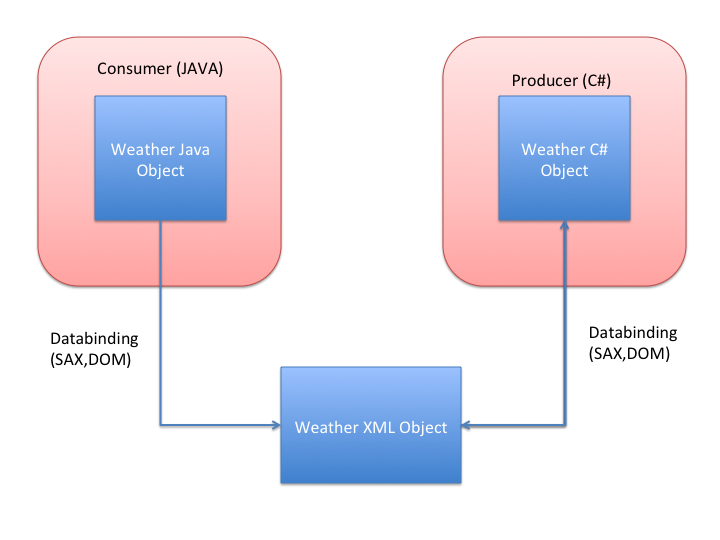
\includegraphics[width=0.8\textwidth]{Figures/databinding.png}
  \caption[Data interoperability.]{Data interoperability.}
  \label{fig:datainteroperability}
\end{figure}

Basically, in these solutions, the receiver needs to be worried with the format and field names of the incoming messages that consumer creates. The target of asymmetric interoperability is removing this coupling problem between consumer and producer.


\subsection{Asymmetric interoperability}
\label{section:asymmetricinteroperabilityProblem}

The implemented approach in new solution proposes to use partial interoperability, based on the concepts of compliance and conformance. It introduces a different perspective, stronger than similarity but weaker than commonality (sharing). The trick is to allow partial interoperability, by considering only the intersection between what the consumer needs and what the provider offers. It allows for increased interoperability,
 adaptability and changeability, without the need to have resource types necessarily shared or previously agreed.
 Building interoperability on compliance and conformance avoids the problem of having to define schemas as separate documents and to agree upon them beforehand. As long as compliance and conformance hold, any two resources can interoperate, even if they were designed unawares to each other. In that solution, consumer will communicate with provider as in current classical solutions, but with a different perspective which avoiding schema sharing. Since there is no shared schema, both consumer and producer can change their structure without informing each other. So consumer and producer do not need to have same structure, Matching will be done field by field between the message and the service operation’s formal argument for necessary fields then in case there is a matching, compliance and conformance will be provided. With asymmetric interoperability the receiver deals with its own format and field names, there is no need to generate a stub to deal with the message (Figure \ref{fig:Asymmetricdatainteroperability}).

 The compliance-based assignment of the message to the receiver’s formal argument is made at binary level, field by field. The receiver deals only with the message format and field names it already knows, instead of having to deal with the whole structure of the message and its field name. This is how it reduces the coupling as long as compliance holds. This is the main advantage of asymmetric interoperability. The disadvantage of this solution that consumer can try to communicate with producer and if there is nothing mapped between the message and the service operation’s formal argument then any operation will be invoked, which means consumer and producer will not exchange the information.

 \begin{figure}[!htb]
   \centering
   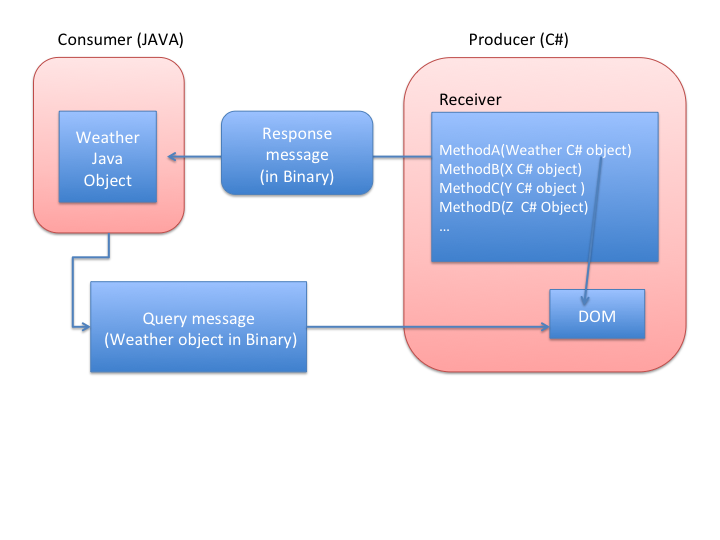
\includegraphics[width=0.8\textwidth]{Figures/compliance.png}
   \caption[Asymmetric interoperability.]{Asymmetric interoperability.}
   \label{fig:Asymmetricdatainteroperability}
 \end{figure}

As seen in the example of section \ref{section:AsymmetricInteroperability}, client or the server without breaking interoperability can change their structure of messages. This brings great facility both client and the server by reducing coupling when compared with current traditional solutions. The example (in Section \ref{section:AsymmetricInteroperability}) also shows that using the asymmetric compliance and structured data, it is equally suitable for both examples of SOA and REST (in Section \ref{section:InteroperabilityData}), allowing both service interfaces and structured resources.
